% vim: foldmethod=marker foldcolumn=3

% {{{ 绪论
\chapter{绪论}
\section{选题依据及意义}

数据中心被目前的企业中所广泛采用,
大型的数据中心甚至承载着公司的服务系统. 其中,
服务器应用程序之间的连接几乎全部是通过TCP/UDP协议.
用户对网络性能的要求日益扩大, 一些微小故障很可能会造成用户体验的下降,
特别是在某些交互敏感的场合, 服务的质量必须得到保证. 可是对于庞大的系统,
各种问题的发生是无法避免的. 我们只能更快, 更精准的解决问题,
以此将故障的损失降到最低, 这也是对新时代的检测调试工具的挑战.

面对大型复杂数据中心的调试以及错误, 如果仍然使用简陋的单机调试手段,
例如\texttt{ping}, \texttt{tracerout}, 也许可以解决问题, 但其代价与耗时,
是无法满足运营要求的. 进而, 许多公司提出了自己的方案,
甚至为自己搭建的集群开发出一套相匹配的网络调试工具.


\section{研究目标和主要内容}

在数据中心网络(DCN)中, 众多网络设备运行过程中的故障在所难免,
及时发现故障并确定故障位置成为DCN网络运维的重要组成部分.
本课题参照微软提出的Everflow故障检测方案,
设计并实现一款面向数据中心网络的流量分析与故障检测工具.

为了解决现实存在的数据中心的网络异常问题, 利用现有商用交换机的
\texttt{Match and Mirror}机制, 将特定的数据包进行镜像.
镜像后的数据包包含了整条链路的信息,
通过链路信息即可分析当前网络中存在的故障.


  在实验室中, 董老师与学长学姐们正在基于专有硬件平台(mips)编写数据包级别的分析器.
本次的设计, 我是基于通用处理器平台(x86-64)进行构建. 在毕业设计进行的同时,
为专有平台的程序编写提供参照.

  程序设计中, 关注于DCN中环路及丢包的检测,
结果保存, 预警, 数据展示, 探针构造几个方面. 在初步实现Everflow功能的基础上,
进行了简单的改进完善, 下面列出了程序的主要功能:

\begin{itemize}
\item
  对实时采集到的数据包进行分析, 实现丢包检测, 环路分析等故障检测;
\item
  采用两阶段的分析方案, 分别为快路径与满路径;
\item
  在分析时, 多处使用hash数据结构来提高查找效率, 以加快处理速度;
\item
  按需保存Trace数据, 以进一步确定故障位置和故障原因;
\item
  支持探针数据报文的发送(需要管理员手动触发)
\item
  采用B/S架构, 管理员通过浏览器即可进行操作
\end{itemize}
% }}}

% {{{ 国内外研究现状
\chapter{国内外研究现状}
\section{数据中心网络故障检测方案}

不论是学校还是企业, 许多都设立了自己的数据中心,
有关数据中心的网络故障检测, 都有自己的见解与考量. 对于更为大型的数据中心网络,
更是有人提出了集学校公司之力, 共同开发系统, 不断的部署与完善.

经过对国内外近期文献的查阅, 我发现,
这些系统或是工具可以按照不同角度进行分类. 在主动性方面,
有主动探测故障的, 有被动触发, 还有使用日志记录来查看的; 在网络层次方面,
有些在数据包层面, 有些则专注于数据流层面; 根据部署位置不同,
也可以分为在交换机部署, 在终端部署, 或者两者均进行部署; 在使用范围上,
有些适合于通用平台, 有些只能适用于某个特定厂商; 在处理上,
有些拥有流水线来处理结果, 有些则是简单的排除错误; 按工具性质来看,
有些属于调试小工具, 专注于某个方面, 也不需要一直在线,
有些则是属于系统级别的服务工具, 为整个DCN所使用, 需要一直在线;
在错误处理上, 有些可以借助控制设备自动进行处理,
而有些则需要向管理员预警, 需管理员手动进行处理. 以下介绍各个方案的一些特点.

Planck: \cite{rasley2014planck} SDN的出现使得自己调节的网络得以实现, 这样
的网络可以实时监控, 并能立即对重要的事件例如拥塞做出迅速反应.
但是目前的监控机制需要数百毫秒来重新探测全局网络, 对于实时的错误,
这样的延迟是很致命的, 这篇2014年的论文提出了新颖的网络测量架构,
使用端口镜像的机制来提取网络信息. 但是可以在相当
短的时间内对网络信息进行获取. 而且不会对网络造成太大的影响.

LossRadar: \cite{li2016lossradar} 属于有针对性的工具,
着重介绍有关丢包的抓取问题. 虽然只是检测丢包,
但是这也足够成为一个检测系统了, 这个工具可以在较快的时间
内抓取单独的丢包以及它们的详细信息. 它需要在交换机上部署,
但是并不需要很多的流量和带宽.

Cherrypick: \cite{tammana2015cherrypick} 一个可扩展的简单的轨迹追踪技术
目前的数据轨迹追踪需要负担大量数据积累的开销,
或是在数据平面大量资源的消耗, 交换机规则或是数据包头部的探查.
它的核心思想是挑选链接, 这些链接是表示数据包端到端路径的关键,
并在到达目的地的路上将其嵌入数据包头部. 通过使用最新的头部标识技术,
它只需要很少的交换机规则即可,

SDN traceroute: \cite{agarwal2014sdn} 使用具有了SDN功能的设备, 不过只要
支持OpenFlow1.0的设备即可. 它可以通过SDN支持的网络中的任意数据包来确定路径,
这个路径使用SDN支持的转发机制, 而且并不需要修改转发规则.
可以探测任意的以太网数据包的转发行为, 以及交换机和控制器逻辑中的调试问题.

PathDump: \cite{tammana2016simplifying}使用了较为不同的方法,
仔细划分了边缘设备与网络元素之间的调试任务.
利用边缘设备的资源进行网络调试的简约工具. 并且可以支持大量网络调试问题.
需要的资源较少, 而且可以在较细的时间粒度调试.

Pingmesh: \cite{guo2015pingmesh}
这个系统已经在微软的数据中心部署了超过4年, 它的理念很简单,
就是想要在任意时刻获取任意两台服务器的延迟信息. 因此, 它的目标就是
去定义一个网络延迟检测和分析系统, 它也需要为所有的服务器产生延迟信息,
因为延迟数据属于基础信息, 能够帮助我们更好的管理网络,
以及解决网络中的问题. 这项服务也必须长期在线, 并保证稳定性.
它可能是最不需要关心路由器等设备的一个方案了, 对于整个系统来说,
知道延迟就是目标, 在实现时, 主要借助了ping的思想,
所有服务器要从中心控制器下载文件, 进行延迟探测后传回中心服务器.
它借助了微软自己开发了存储系统, 也实现了 数据处理流水线.
相比于之后提出的Everflow, 它更像是微软的第一代产品, 稳定而强大.

NetSight: \cite{handigol2014know}, 这是一个完全记录网络历史的工具.
在文章中, 介绍了如何使用packet histories(每个包的整条记录)来简化网络的调试.
为了展示\texttt{packet\ histories}的作用, 以及实现上的可行性,
创造了\texttt{NetSight}, 一个可扩展的平台,
允许程序简便的检索网络的历史状况. 在\texttt{NetSight}上, 有4个程序:
可交互的网络调试器, 实时的监视器, 一个历史记录器, 一个分级分析器.
在一个现代的多核服务器上,
\texttt{NetSight}可以在10G/s的链接中处理历史包. 对于更大的网络,
它可以通过增加服务器或是硬件或是交换机的数量来扩展. 需要借助SDN,
支持Openflow的交换机才能配合工作, 由于其记录了数据包的历史, 所以
能最大程度还原当初的网络模型, 也因此会给网络带来高负荷, 性能也会损失,
当然也可以通过增加硬件来进行提升. 这是一个与Everflow较为相似的产品,
Everflow中对其一个重要的改进就是增加了匹配模式, 对特定的历史包生成记录,
能有效减少网络负载, 以及处理难度.

Netography: \cite{zhao2016netography} 这也是一种基于软件定义网络(SDN)的
一个工具, 之前的工作关注于静态检查, 被动监控, 以及活动探针,
这些依赖于控制设备以及网络设备的抓取规则. 它定义了一个数据包行为的概念,
用以描述数据包的真实变化, 并强调对故障排除的重要性. 基于通过
由主动发送的探测器触发的副本导出分组行为和流规则的新颖方法,
提出了Netography系统, 并说明了关于转发错误时的排除任务过程,
以及由非租户争用造成的性能下降问题.

Dissecting RTT(round trip time): \cite{marchetta2014dissecting} 与其说它
是工具, 不如认为这一种技术, 利用单个数据包探测延迟的技术. 研究人员
与操作者经常会在监控, 故障排除, 或是其他方式访问网络路径时测量往返时间.
因为延迟时间中结合了所有跳的过程以及转发和反向路径,
所以很难去衡量特定网络元素的延迟.
在这项工作中, 提出了一种新的方法: 在区块中, 映射特定路径后
基于单个数据包探测往返延迟. 使用针对中间路由器的IP Prespecified
Timestamp选项, 它可以提供慢速路径部分的往返时间估计.
这个技术在Everflow中也被用到了, 用于探针方法测量时延.

Passive Realtime Datacenter: \cite{roy2017passive} 这是在Facebook的数据
中心上进行测试的一种方案, 它不去简单的观察异常现象,
而是考虑异常对整个系统的性能所造成的影响. 虽然是基于这么一种简单的设想.
但其实现需要深深结合数据中心的架构. 他们开发了轻量级的包标记技术,
仅仅使用转发规则(交换机支持). 作为路径中唯一标示. 文章中对于现有IPv6头部, 
还很难寻求一份区域用于调试.


\section{Everflow简介}

  Everflow \cite{greenberg2016packet} 这是微软在2015年发表在
SIGCOMM的论文中提出的方案. 与部署运行超过了4年的Pingmesh\cite{guo2015pingmesh}
不同, 它并没有特别关注端对端的延迟, 而是从数据包层面进行分析.

  对于Everflow来说, 最大的挑战莫过于扩展性了. 大型DCN(10W以上的服务器)中流量
轻松就能达到100Tbps, 追踪这样规模的数据包需要大量的网络资源与服务器资源,
想象一种典型的情况, 平均每个包的大小为1000bytes,
每个镜像数据包64bytes(只包括头部信息), 并且网络的直径为5跳. 如果我们
简单的追踪每个数据包的每一跳作为数据包历史, 数据流量就会有这么多
$\frac{64B}{1000B} \times 5(hops) \times 1000(Tbps) = 32(Tbps)$, 如此高的追踪流量
将会造成网络拥塞和丢包, 特别是当网络利用率很高时.

  另一个扩展性的挑战是路径分析. 因为商用交换机有限的存储与CPU运算能力, 追踪数据包
必须由服务器来完成. 即使假设一个服务可以处理10Gbps的流量, 我们需要
$\frac{32Tbps}{10Gbps} = 3200$这么多服务器来处理, 这也是很大的开销.


\begin{figure}
  \centering
  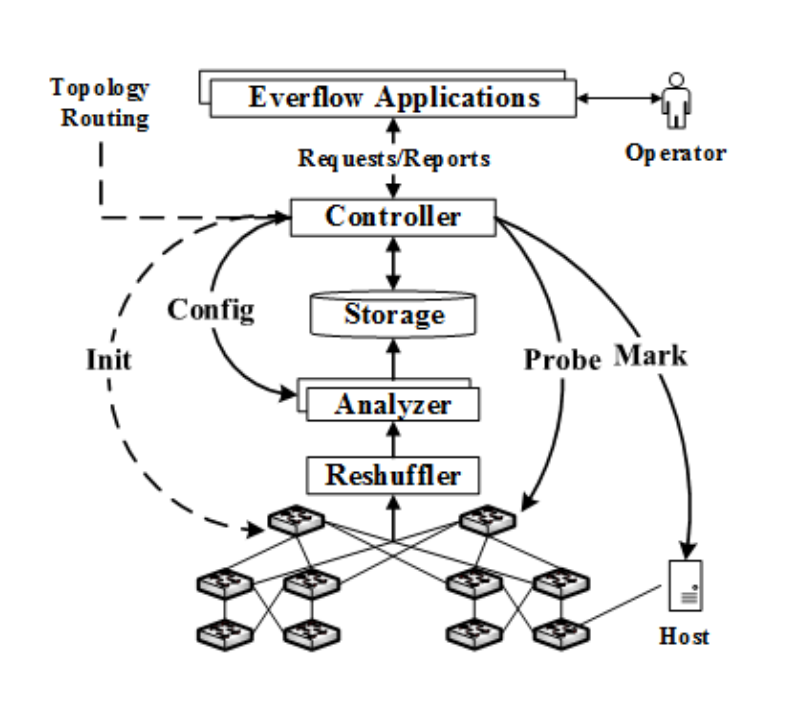
\includegraphics[width=0.58\textwidth]{../img/everflow_arch.png}
  \caption{Everflow的路径收集与分析流水线}
  \label{fig:everflow_arch}
\end{figure}

  如图\ref{fig:everflow_arch}所示为Everflow的架构.它由四个主要组件组成:
控制器, 分析器, 存储器以及洗牌器. 在顶层, 有许多应用程序使用由Everflow提供的信息
去调试网络错误. 控制器负责协调其它组件以及和应用程序交流. 在
初始化过程中, 它配置交换机上的规则. 被匹配到的数据包将被镜像至洗牌器, 而后会直接
到达分析器中, 分析完成后, 分析结果将传递至存储器中.
控制器也提供了一些API, 允许Everflow的应用程序去查询分析结果, 并且在主机上设置debug位.

  Everflow的关键思想在于镜像特定的报文, 在商用交换机上设置特定的匹配规则, 将匹配后的数据包发出.
而后利用交换机内置的ASIC芯片的负载均衡, 捕获到的数据包
会被重新分发到不同的分析服务器上, 通过五元组信息(源IP, 目的IP, 源端口, 目的端口, 协议类型)
能保证在同一轨迹上的数据包能分发至相同的服务器上,
它也能发送定向探针去确认潜在的错误.

  2014年, 微软工作人员在微软两个的数据中心上进行Everflow部署.
第一个部署的是前期制作的集群, 其中有37台交换机. 第二个部署是对生产环境的
2500台交换机中的440台进行部署. 两个集群承载了许多应用程序的流量.
除此之外, 工作人员也在特定的生产交换机上开启了Everflow, 用以支持在线错误的调试.
目前, 微软工作人员也扩展了Everflow的部署以使其可以被更多的交换机和集群使用.
通过部署在微软的DCN上, Everflow证明了其作为诊断DCN错误不可或缺的工具的实用性.
% }}} Everflow简介

% {{{ 流量分析与故障检测总体方案
\chapter{流量分析与故障检测总体方案}

本文实现的流量分析与故障检测方案包括三大部分: 分析器, 控制器, 以及访问页面, 以下分别进行概述,
更加详细的实现细节请查看接下来三章的设计方案.

\begin{figure}
  \centering
  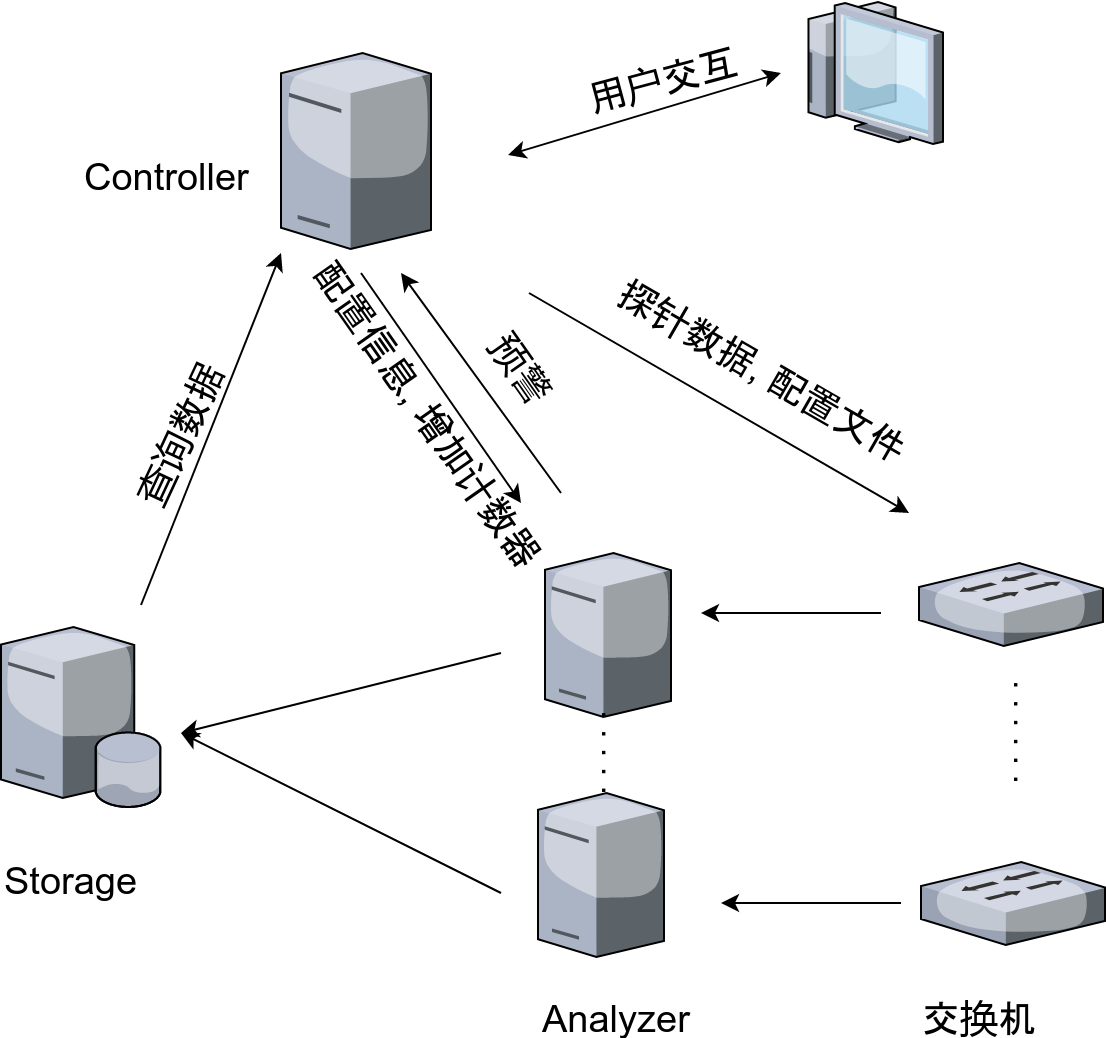
\includegraphics[width=0.55\textwidth]{../img/user_flow.png}
  \caption{架构设计}
  \label{fig:arch}
\end{figure}

图\ref{fig:arch}为整个系统的结构. 镜像后的数据包传递至分析器中, 分析器检查过后,
异常的数据以及统计结果将会保存在存储器中, 用户可以通过访问页面来查询问题数据.

\section{分析器功能设计}

  分析器是分布式的服务器, 且每个服务器处理一部分流量数据.

  对于特定模式的数据包进行统计, 通过统计数据, 可以获得当前网络中的流量状况.

  在分析器中, 我们期望获得的是在DCN中数据包的完整路径. 对于存在问题的路径信息,
我们可以得知是否有环, 或是有丢包现象, 存在以上问题的路径信息将会存储至存储器中.

  对于探针来说也可以粗略衡量交换机之间的延迟.

\section{存储器功能设计}

存储器中, 主要存储分析器产生的结果, 包括网络流数据与相应规则的统计数据.
本方案中, 使用关系型数据库MySQL\cite{mysql}进行数据存储.

网络流数据表格中, 每一行数据对应给一个追踪记录,
包括数据包的原始信息(第一个数据包的达到时间, 五元组信息),
数据包的多跳信息, 当前网络流的元数据信息(是否有环, 是否丢包, 是否为探针).
对其中一些信息, 可以在查询时可以指定规则来进行过滤查找.

我们也在表格中存储了所有分析器产生的计数值, 表中的每一行代表着从分析器取得的
一条计数信息, 包括计数器的ID, 记录时间, 分析器ID.

同时, 存储器中, 也存储了全部的统计规则.

\section{控制器功能设计}

控制器有几个主要功能: 对分析器配置, 向外提供API接口, 向交换机中发送探针.
目前我们提供的API包括: 按时间查找数据流, 查询计数器的值, 添加探针,
发生错误后的预警功能.

\section{访问页面功能设计}

此部分用于展示存储器中的数据, 包括网络流数据, 不同的规则下的统计数据.
另外提供用户与程序的交互接口, 包括增加删除统计规则, 探针的构造及发送.

\section{技术选型}

根据对性能的不同要求, 结合开发进度做如下讨论. 在分析器中,
需要考虑大量的流量涌来, 必须充分利用系统资源进行数据包的接受和处理,
使用偏向底层的C/C++语言, 在控制器中, 只涉及简单的数据库查找与用户交互,
对性能要求不高, 故使用Python, 以实现迅速而敏捷的开发.

对于本次的系统设计, 分工如下:

\begin{itemize}
\item
  分析器采用C/C++完成
\item
  选择关系型数据库MySQL作为存储器
\item
  控制器通过Python实现, 与用户的接口采用HTTP协议交互
\item
  访问页面采用HTML+CSS+Javascript实现,
  其中, 图表展示打算使用开源的echarts.
\end{itemize}
% }}}流量分析与故障检测总体方案

% {{{ 实现方案
% {{{ 分析器实现方案
\chapter{分析器的设计与实现}

\section{算法设计}
\label{sec:分析器主要算法说明}

\textbf{环路检测算法}: 环路检测是设计中最为基本的功能, 目前的程序中只是做简单的环路检测:
 遍历数据路径的所有节点(交换机ID), 如果存在相同的节点, 那么认为此路径中有环.

\textbf{检测丢包算法}: 查看路径的最后一跳是否与我们期望的最后一跳相同.
最后一跳的交换机是无法直接计算得到的, 需要根据数据中心的网络拓扑进行分析.
当前程序中, 控制器下发出口交换机的ID信息,
任何数据包路径中均需要包含两个出口交换机, 我们才能认为它没有在网络中被丢弃.


\textbf{使用探针检测任意交换机的延迟}: 这是一个比较具有考量的方法.
需要交换机具有解封和转发能力.

首先介绍如何实现一跳的探针: 假设我们想要将数据包p发往S,
我们首先根据p构造出\(p^{'}\) 其中\(p^{'}\)的目的IP为S,
而后将\(p^{'}\)发送出去, 当它到达交换机S后, 数据包中的
目的IP与S的IP相同, 则将数据包\(p^{'}\)进行解封操作, 将其还原为p,
再使用正常的转发规则处理p.

实现了一跳的探针后, 可以考虑将探针进行拓展,
使其按找我们理想的路径进行传递, 方式也不难理解,
就是一层层的进行数据包封装, 这样数据包到达交换机被解封后, 就可以
根据内层的数据包进行正常转发了, 从而达到内层数据包所要去的地址中.
对于端到端的延迟, 例如我们想要知道\(S_{1}\)到\(S_{2}\)的往返延迟,
需要对原始数据包进行封装: 第一层, 以\(S_{1}\)的IP为目的IP, 第二层,
以\(S_{2}\)的IP为目的IP, 第三层, 再次将\(S_{1}\) 的IP作为目的IP.
数据包就会按照\(S_{1} => S_{2} => S_{1}\)的方式进行传递. 我们
可以通过此种方法得到粗略的往返延迟.

为什么说粗略呢, 这里,
并不是在交换机\(S_{1}\)上直接获取到了两次数据的间隔时间,
我们只能得到到达分析器的时间, 因为认为\(S_{1}\)到分析器来回路径是一致的,
因此可以 简单的使用分析器获得的两个时间相减得到粗略的往返延迟.

\textbf{定时器功能的实现}:

图\ref{fig:hash_backet}介绍了定时功能的实现, 每经过1s三个数据桶进行一次状态转移.
以0s到1s的时间段为例, 在此时间段内达到的数据包首先检查桶H0, 判断它的trace数据是否
属于H0, 如果属于, 则加入到桶H0中, 否则放置在桶H1中. 待1s结束, 到达1s到2s的时间段后,
我们将桶的状态进行转移, H0中的数据就可以作为慢路径的输入进行处理,
因为桶中的每条trace数据已经包含了整整1s的数据包.

\begin{figure}[htbp!]
  \centering
  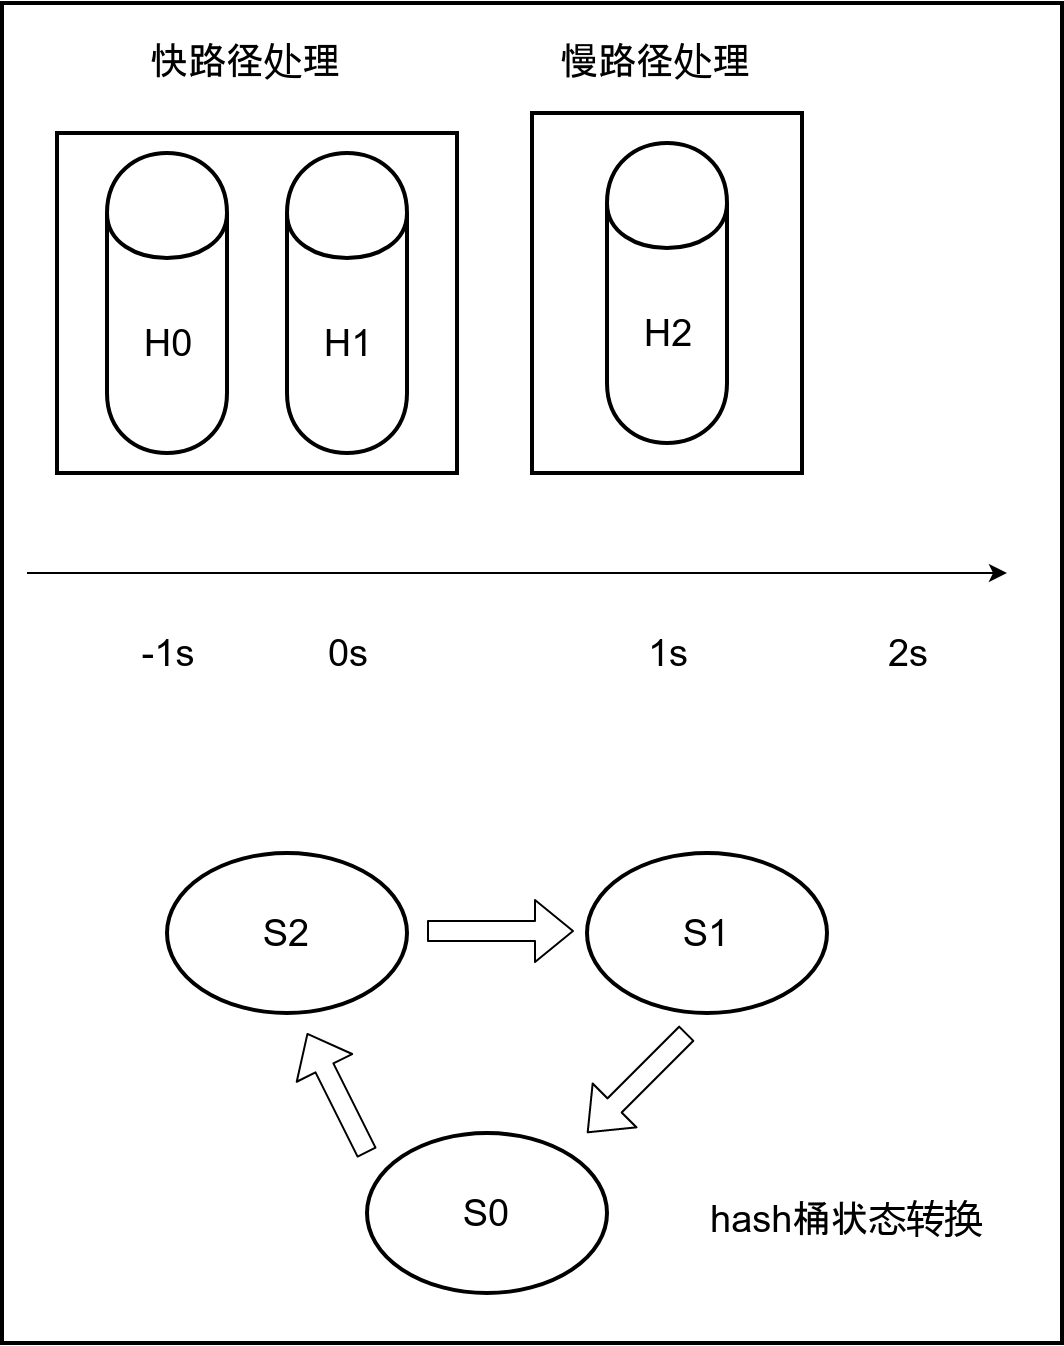
\includegraphics[width=0.8\textwidth]{../img/hash_backet.png}
  \caption{hash桶设计}
  \label{fig:hash_backet}
\end{figure}


  根据图\ref{fig:hash_backet}中的状态转换方式, 设计如下两个线程, 分别进行快慢路径的
处理. 将定时器放在了快路径线程中, 通过定时器的触发来推动状态转换. 如果慢路径的
处理时间过久, 快路径部分将会被\textbf{while(!is\_slow\_over)\{\}}这样的自旋锁所阻塞,
反之也是如此. 目前程序中加入了对自旋锁阻塞情况的统计, 用以确定和解决程序的瓶颈.

\begin{lstlisting}[caption=数据结构,frame=tlrb]{Name}
hash_backet* H0, H1, H2;    // 三个hash数据桶
bool is_slow_over = true;   // 标示慢路径是否完成处理
Mutex lock;                 // 互斥锁, 防止快慢路径同时对数据进行修改
\end{lstlisting}

\noindent\begin{minipage}{.55\textwidth}
\begin{lstlisting}[caption=快路径线程,frame=tlrb]{Name}
clock_t start = clock();
while(!stop) {
  p = GetPacket();
  if(H0 found trace) {
    将p添加至H0中;
  } else {
    将p添加至H1中;
  }

  // 超过1s
  while(clock() - start > 1000)
  {
    // spinlock 检查慢路劲处理是否结束
    while(!is_slow_over){}
    TMP = H0;
    H0 = H2;
    H2 = H1;
    H1 = TMP;
    {
        MutexLock;
        is_slow_over = false;
    }
    // 更新clock
    start = clock();
  }
}
\end{lstlisting}
\end{minipage}\hfill
\begin{minipage}{.38\textwidth}
\begin{lstlisting}[caption=慢路径线程,frame=tlrb]{Name}
while(!stop) {
  while(is_slow_over){}
  // 处理慢路径

  {
    MutexLock;
    is_slow_over = true;
  }
}
\end{lstlisting}
\end{minipage}

\section{数据结构}

\textbf{GRE数据包}

\begin{figure}[htbp!]
  \centering
  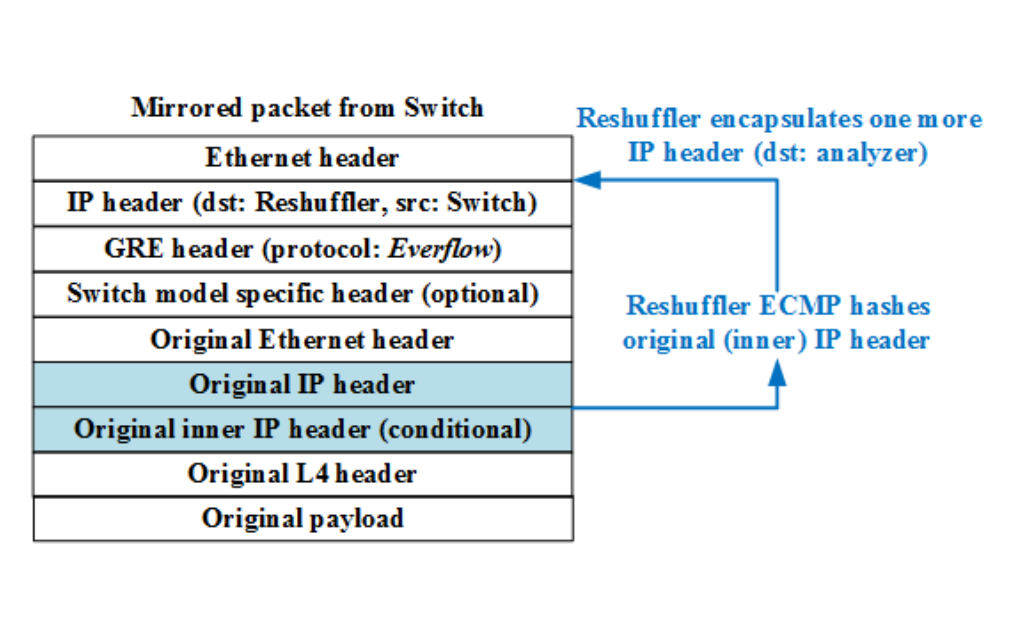
\includegraphics[width=0.65\textwidth]{../img/format_gre.png}
  \caption{GRE数据包结构}
  \label{fig:gre_packet}
\end{figure}

对于到达分析器的数据包来说, 均是使用GRE(Generic Routing Encapsulation)
进行封装, GRE格式见图\ref{fig:gre_packet}.

\textbf{Trace数据}

这是分析器中存储结构: 传入分析器中的是一个个单独的数据包.
在分析器中, 相同路径上的数据包最终使用的trace数据结构来表示. trace数据结构中,
包括数据包内容(数据包内容在路径上都是相同的, 所以保存一份即可)这样的原始信息,
每一跳经过的交换机ID, 每一跳的到达时间, 元数据信息(是否环路, 是否丢包, 是否为探针).

\label{trace数据结构}
\begin{lstlisting}[caption=Trace数据结构,frame=tlrb]{Name}
typedef struct{
    struct in_addr ip_src; /**< 32bits 源IP地址   */
    struct in_addr ip_dst; /**< 32bits 目的IP地址 */
    uint16_t ip_id;        /**< 16bits 标识符     */
    uint8_t protocol;      /**< 8bits  协议字段   */
} __attribute__((packed)) IP_PKT_KEY_T;

enum {TRACE_CNT = 5};   /**< 只记录5跳信息 */

/**
 * @brief trace数据结构
 */
typedef struct{
    IP_PKT_KEY_T key;

    uint16_t pkt_size;   /**< 16bits 数据包大小  */

    /**
     * 32bits 收到第一个报文的时间戳: 如果使用秒级的计数单位, 是无法刻画出真实
     * 的数据包的时间情况, 这里的时间戳是毫秒级别的时间戳,
     * 记录的是基于当天0点偏移的毫秒数.
     *
     *  Timestamp记录收到报文的时间,
     *  如果对于某一跳交换机超过1秒还没收到其它的报文, 则视为丢包
     */
    uint32_t timestart;

    struct {
        uint16_t switch_id: 12;
        uint16_t hop_rcvd : 2;
        uint16_t hop_timeshift: 10; /**< 与timestart相减得到的偏移, 也为ms */
    } __attribute__((packed)) hop_info[TRACE_CNT - 1];

    uint16_t hp1_switch_id: 12; /**< 第一跳交换机id          */
    uint16_t hp1_rcvd: 2;       /**< 第一跳交换机收到的报文数  */
    uint16_t used: 1;           /**< 以hash表进行存储,
                                     记录hash表中的当前元素是否被占用. */

    uint16_t is_loop: 1;
    uint16_t is_drop: 1;
    uint16_t is_timeout: 1;
    uint16_t is_probe: 1;

    uint16_t reserved : 5;
} __attribute__((packed)) PKT_TRACE_T;
\end{lstlisting}


除此之外, 分析器中还有计数器, 记录每个规则下的数据包个数.

在程序中, 需要经过快路径, 慢路径两个处理过程, 由快路径处理结束后,
进入慢路径.

下图\ref{fig:analyzer_process}是具体处理过程. 首先进行
对GRE数据包的解封操作, 解封后,
具有相同标识(通过五元组hash计算得出)的数据包会进入相同的线程中.

\begin{figure}
  \centering
  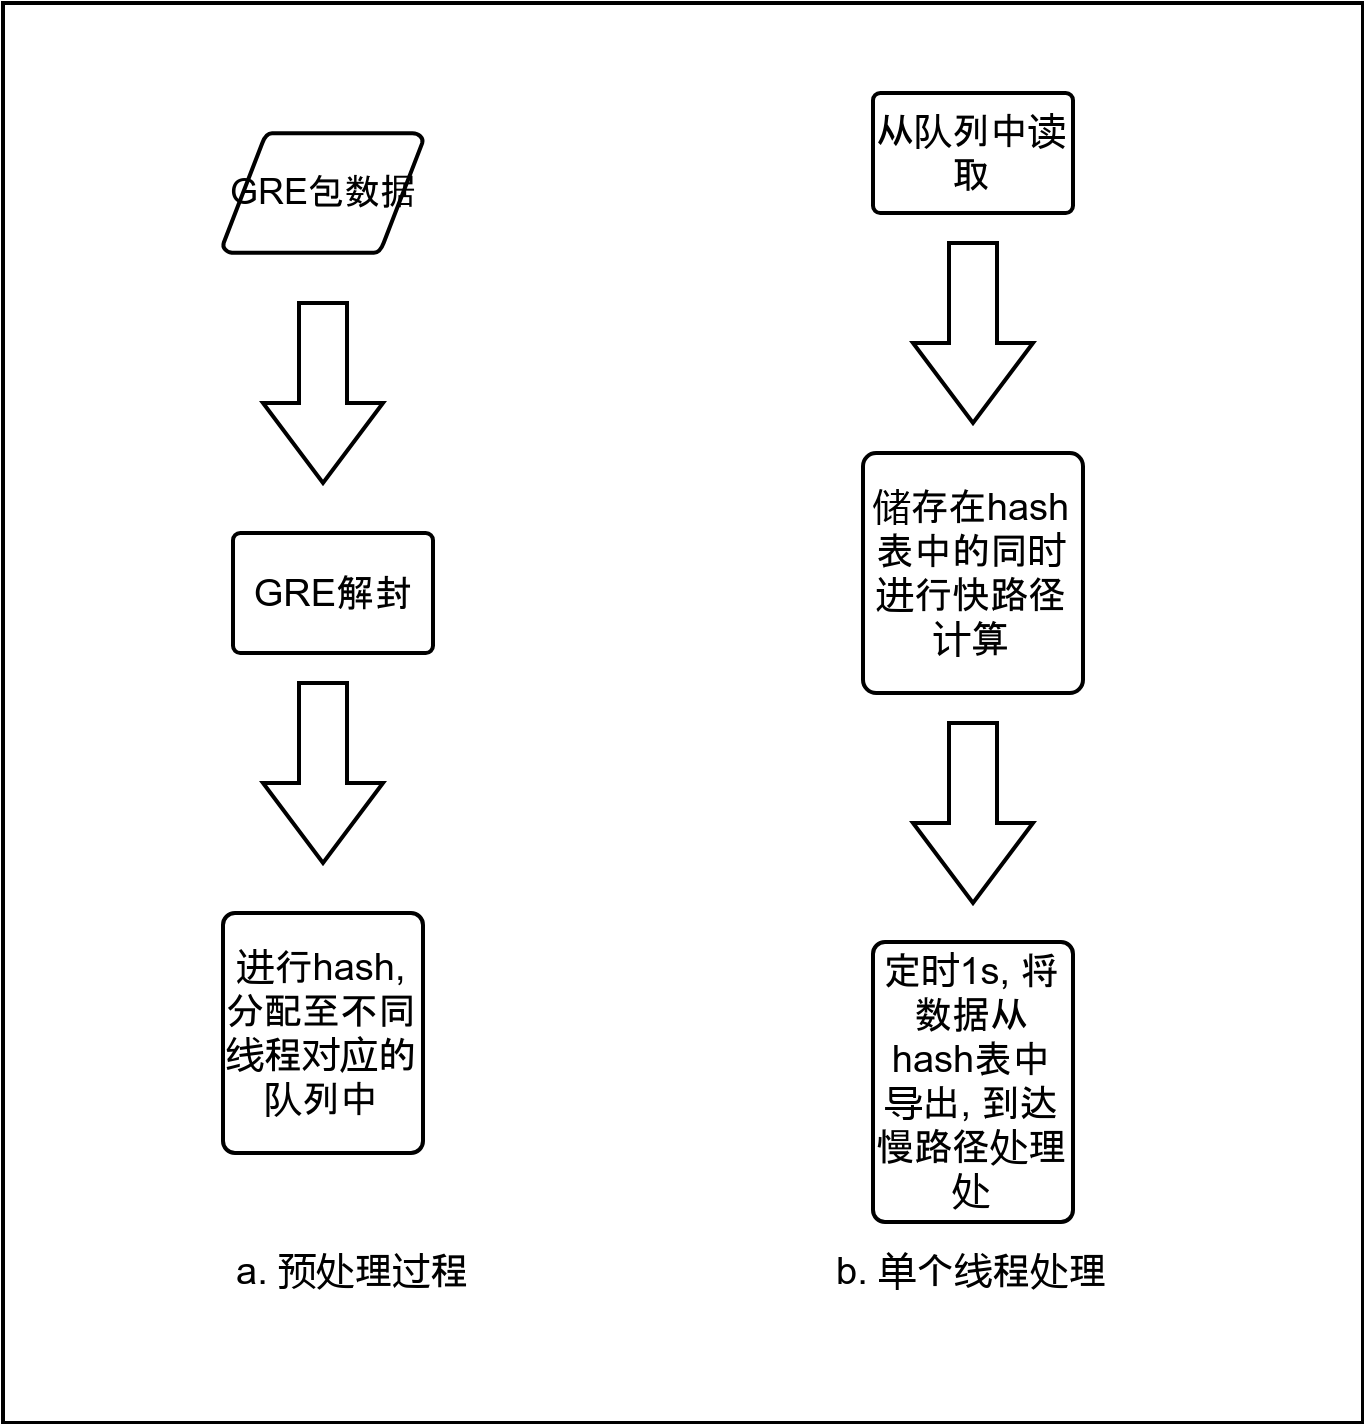
\includegraphics[width=0.6\textwidth]{../img/analyze_process.png}
  \caption{分析器处理逻辑}
  \label{fig:analyzer_process}
\end{figure}

上述的流程图只说明执行顺序, 以下图\ref{fig:analyzer_arch}为程序实际的处理流程,
英文关键字均为程序中确切的类名. 其中, Reader与Processer均可以自行配置个数.

\begin{figure}
  \centering
  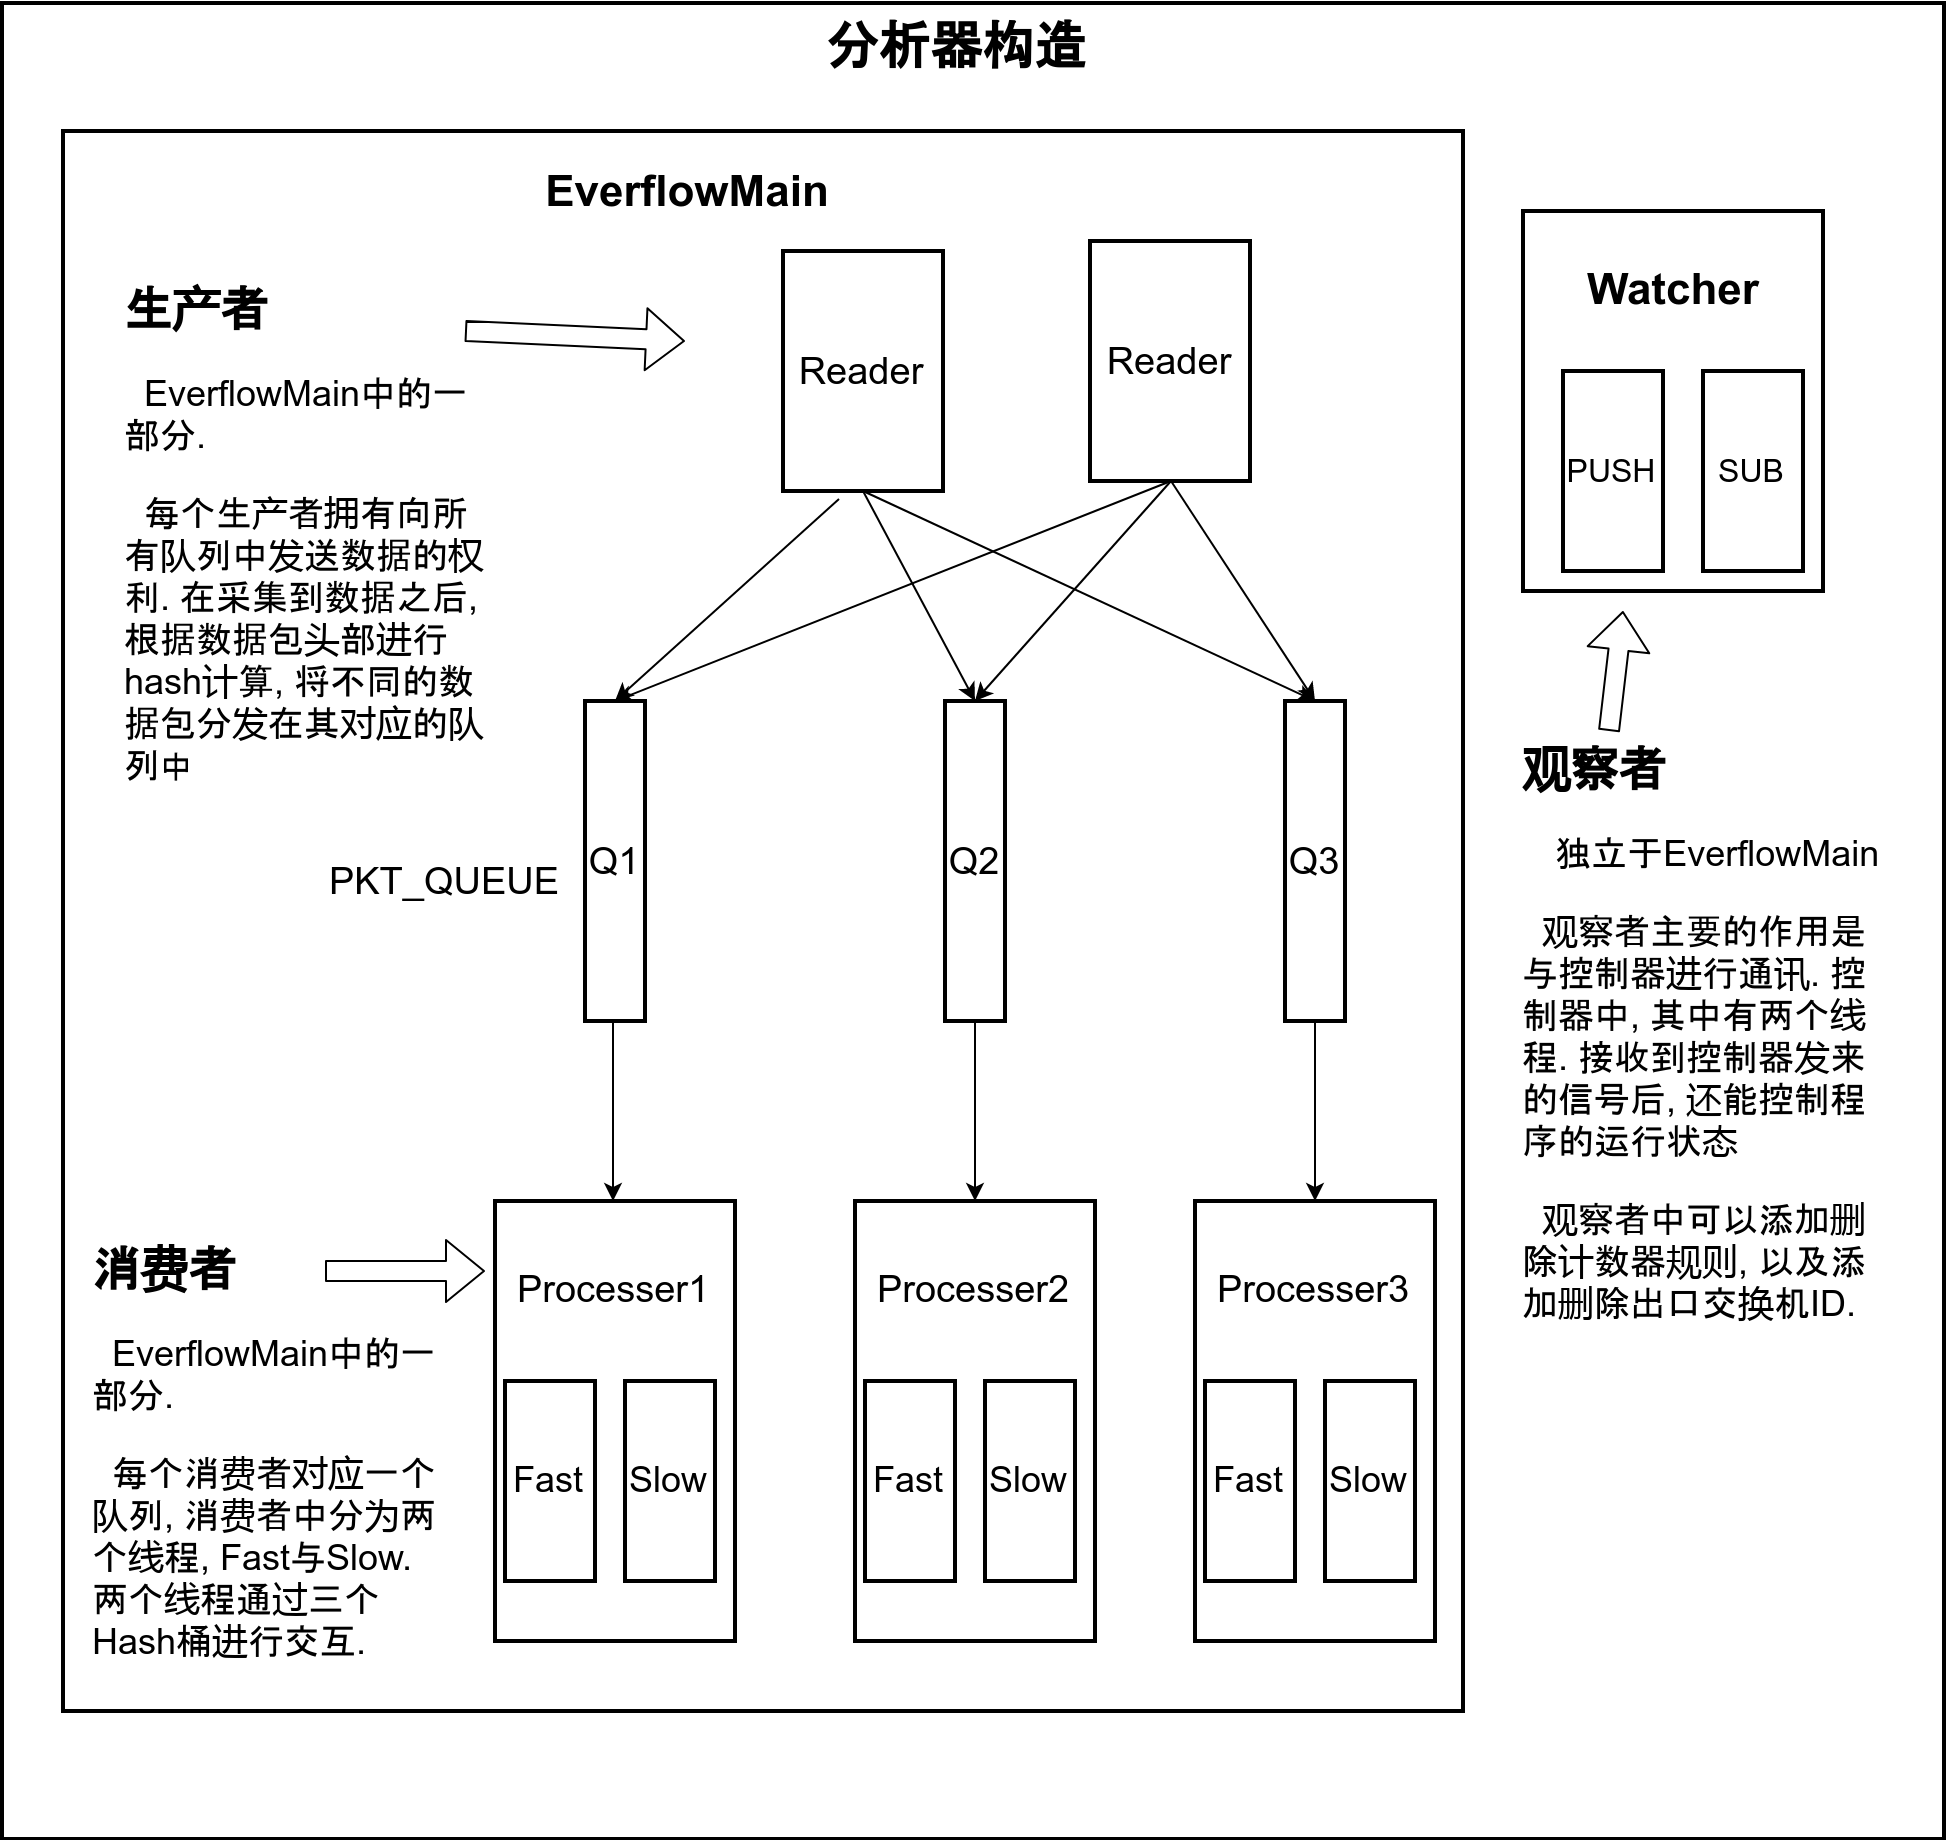
\includegraphics[width=0.9\textwidth]{../img/analyzer_structure.png}
  \caption{分析器架构设计}
  \label{fig:analyzer_arch}
\end{figure}

\section{启动及退出流程}

\subsection{程序启动流程}
\label{sec:分析器启动过程}

  启动时, 首先初始化\texttt{Watcher}, 继而向控制器发送\texttt{INIT}信息,
请求出口交换机ID信息与当前的的统计规则. 收到控制器的回复后,
启动\texttt{Processer}, 而后启动\texttt{Reader}, 这
时的\texttt{Reader}开始获取\texttt{GRE}数据包, 并根据内层的五元组进行hash操作,
按结果存入到相应的队列中, 供\texttt{Processer}使用.

  在向控制器发请求时, 分析器必须带上自己的ID作为请求标识.
在控制器处理结束后, 返回的报文中也会携带有分析器的ID, 所有的分析器获取到广播后,
对比收到的响应报文中分析器ID与自身ID. 如果ID相同, 则说明是对自己的操作, 否则
丢弃该报文.

  另外, 对于返回报文中ID为0的情况, 这是一种广播的形式, 所有的分析器必须按照广播
报文进行操作.

\subsection{程序退出流程}

程序停止时, \texttt{Watcher}首先向控制器发送\texttt{QUIT}信号,
通知控制器, 当前的分析器准备停止了, 而后, 控制器做出回应.
每个控制器下监管许多分析器, 它有权也应当知道所有分析器的状态.

程序中多次使用了队列进行解耦, 如果队列为空, 那么所有的消费者将会被阻塞.
程序收到退出信号后, 一定是先将生产者全部停止, 待生产者全部停止后.
向队列中发送截止数据包, 向消费者表明生产者已经不再继续生产了,
可以停止了. 消费者会将当前队列中的数据包消耗完毕, 而后停止.

\section{分析器实现中遇到的问题及解决方案}

\subsection{毫秒级时间戳的使用}

我们通常所说的时间戳,
是指1970年01月01日00时00分00秒(北京时间1970年01月01日08时00分00秒)起至现在的总秒数.
是以秒为计数单位的.

在我们的trace数据结构中, 也采用了32位整数作为时间戳, 但是针对网络中的数据包. 它们的
传播速度是在微妙级别, 用秒做单位根本无法进行时间估计.

\subsubsection{可能的方案}

考虑过之后, 有以下两种方案:

\begin{itemize}
\item
  再来32位, 表示毫秒.
\item
  将原始的方案中时间戳的含义更改,
  使其表示从一个特定时间开始经过的总毫秒.
\end{itemize}

第一种方案, 需要修改原先的数据结构了, 向其中增加4个byte,
虽然我们目前的程序不是针对嵌入式的设备, 但是需要克勤克俭用CPU缓存,
具体的数据结构在\ref{trace数据结构}已经列出. 根据我们的定义情况,
假如每个对象增加了4个字节, 原始的128byte的CPU缓存就不够存放4个trace了,
会造成性能下降.

第二种方案, 从特定时间开始, 记录基于这个时间的偏移, 那么就会产生一个问题:
32位(大约有20亿)的时间戳以毫秒为单位, 到底能够表示长时间.

这里计算了32位的数据能表示的天数.

$$ \frac{2 \times 10^{9} ms }{24 \times 3600 \times 1000} = 23 Days$$

粗略的计算表明, 如果使用毫秒表示时间戳, 最多也就只能表示23天,
如果使用\texttt{unsigned\ int}, 时间翻倍也就是46天,
如果使用每一年的年初作为起始, 偏移最多能表示46天, 完全达不到我们的要求.

\subsubsection{最终方案}

使用32位时间戳表示当天偏移的毫秒数, 再加一个字段保存日期.
但这个字段不放在分析器的trace结构中, 而是放置在数据库里.

采用这个方案的原因有以下两点:

\begin{enumerate}
\def\labelenumi{\arabic{enumi}.}
\item
  32位的时间戳已经足够表示1天内偏移的毫秒数.
\item
  整个系统的实时性很强, 误差也不会超过10s, 存入数据库时,
  将数据库当天的日期作为 日志日期写入到字段中, 这样,
  可以保证我们在搜索时获得正确的时间戳, 也不需要考虑空间占用问题, 并且,
  这个新增的日期字段可以作为索引来使用.
\end{enumerate}

日期字段可以通过MySQL的trigger进行设置.


\begin{lstlisting} [caption=Triger设置]{SQL}
CREATE TRIGGER `fdate_set` BEFORE INSERT ON `tbl_trace_data`
FOR EACH ROW BEGIN
  SET NEW.fdate = CAST( DATE_FORMAT(NOW(),'%Y%m%d') AS UNSIGNED);
END
\end{lstlisting}

\subsubsection{细节问题}

这样存储会有一个问题: 如果出现了快到第二天0点时存入了数据,
而设置日期时已经到了第二天 例如: 2018-03-22 23:59:55 时准备存入数据库,
之后数据库中的fdate被设置为了2018-03-23, 这是一种不匹配.

这个问题也有解决方式: 可以通过判断时间戳的偏移, 如果偏移过大, 则认为它是
第一天的数据, 也就是03-22的数据, 上面只是列了最简单的Trigger设置.

\subsection{热重启与容灾问题}
\label{sec:热重启与容灾问题}

在考虑到控制器与分析器的交互后, 直接启动分析器的情况已经在
分析器启动过程\ref{sec:分析器启动过程}中提到这个问题,
但是作为线上项目, 热重启与容灾也成为了一个问题.

目前, 我的打算是将分析器部署在五台服务器上, 线上有三台分析器, 另有两台分析器进行容灾.

\subsubsection{热重启}

重启过程是一个分析短暂暂停的过程, 即使我们想要使其继续接受流量,
我们也要做好分析速率变慢的准备.


进行重启操作时, 采用分批重启的形式. 假如我们需要热重启分析器1,
首先配置交换机, 将网络流量导入到分析器2,3中, 重启分析器1完成后,
再将流量导入到分析器1,3中, 依次类推. 如果容灾机器空闲,
可以考虑导入先导入到容灾机器中.

\subsubsection{容灾}

当分析器遇到了故障, 需要检测时, 首先启动容灾服务器, 继而修改交换机配置,
将故障分析器的流量全部切换到容灾分析器后, 停机检测.

\subsection{定时器与signal}

在当前的程序中, 定时上传功能可能只需要10s, 或是20s才上传一次,
单独开线程进行上传操作显得十分浪费.

最终, 我决定使用Linux中的定时器功能. 配置程序, 使得Linux
定时向程序发送\texttt{SIGALRM}信号,
这样, 我们在信号处理函数中添加上传操作即可.

不过, 这样做会造成一个问题, POSIX的信号处理函数只接受一个参数,
我们需要使用全局变量才可以在信号函数中访问程序中的数据.

\subsection{与控制器的交互部分}

与控制器的交互分为两个部分, 发送和接受. 这两个部分均在watcher中实现.

\textbf{发送}: 向消息队列中发送信息, 该消息队列由向控制器监听.

使用消息队列主要是因为可能有多个分析器需要上传请求, 队列是一个比较简单的方式.

\textbf{接受}: 从某个频道中读取控制器命令, 如果是属于自己的命令信息, 则进行相应操作.

如果控制器采取一对多的连接方式, 其实是没多少必要的, 与分析器交互主要是增加删除规则,
增加删除出口交换机ID, 而这样的操作基本是对所有分析器进行的. 使用
订阅-发布模式可以简化控制器的逻辑, 提高效率, 并且有利于分析器数量上的扩展.

与控制器的交互部分全部采用\texttt{Redis}解耦,
其中使用了\texttt{Redis}的\texttt{消息队列}和\texttt{订阅发布}两种接口.
两种接口的使用与调试方式如下:

\textbf{消息队列}: 由 分析器 =\textgreater{} 控制器

\begin{lstlisting} [caption=分析器推送]{Name}
> 127.0.0.1:6379> LPUSH foo 1234 # 分析器PUSH
> (integer) 1

> 127.0.0.1:6379> LPOP foo  # 控制器接受
> "1234"
\end{lstlisting}


\textbf{Pubsub}: 由控制器发送广播, 许多分析器监听相同的频道


\begin{lstlisting} [caption=控制器下发]{Name}
> 127.0.0.1:6379> SUBSCRIBE foo        # 首先启动监听foo频道 
> Reading messages... (press Ctrl-C to quit)
> 1) "subscribe"
> 2) "foo"
> 3) (integer) 1
> 1) "message"
> 2) "foo"
> 3) "12334"

> 127.0.0.1:6379> PUBLISH foo 12334   # 控制器向foo频道中发送
> (integer) 1
\end{lstlisting}



% }}} 分析器实现方案

% {{{ 控制器的设计与实现
\chapter{控制器的设计与实现}

\section{控制器与分析器的接口设计}
\label{sec:分析器, 控制器接口设计}

\subsection{启动过程}

每台分析器启动时, 首先向控制器发送请求. 获取计数器规则, 以及出口交换机ID,
这里是向控制器监听的队列中发送初始化请求.

\begin{lstlisting}[caption=分析器初始化请求]{Name}
{
  "ACTION": "INIT",
  "ANALYZER_ID": 124         // 分析器ID, 由分析器的配置文件进行配置
}
\end{lstlisting}

控制器收到报文后, 针对当前的分析器ID, 进行返回, 同时带上出口交换机的ID,
以及计数器信息, 通过控制器进行配置, 可以简化分析器部分.

\begin{lstlisting}[caption=控制器返回报文]{Name}
{
  "ANALYZER_ID": 124,           // ID为0, 表示这是一种广播操作.
  "MESSAGE": {                  // 报文主体
    "COMMOND": "INIT",          // 初始化
    "SWH_ID": [
        14, 23, 19, 40
    ],
    "COUNTER": [                // 计数器的filter
        {
            "CNT_ID" : 10,
            "SRC_IP": "192.118.0.2",
            "DST_IP": "192.119.0.1",
            ...
        }
    ]
  }
}
\end{lstlisting}

\subsection{更新出口交换机与计数器信息}

由控制器主动进行发送指令, 触发分析器的重载过程, 重载会导致分析速率下降,
在热重启与容灾部分\ref{sec:热重启与容灾问题}提供了一种解决方案.

\begin{lstlisting}[caption=控制器下发指令]{Name}
{
  "ANALYZER_ID": 13,        // ID为0, 表示这是一种广播操作.
  "MESSAGE": {              // 报文主体
    "COMMOND": "RELOAD",    // 重载过程, 这里认为是热重启
    "SWH_ID": [
        14, 23, 19, 40
    ],
    "COUNTER": [            // 计数器的filter
        {
            "CNT_ID" : 1
            "SRC_IP": "192.118.0.2",
            "DST_IP": "192.119.0.1"
        }
    ]
  }
}
\end{lstlisting}

增加删除Counter规则, 以及出口交换机ID, 这一操作应该是针对每个分析器进行, 以下为
具体的命令. 表\ref{tbl:message}列出了所有可用的接口形式.


\begin{table}[]
    \centering
    \caption{控制器命令}
    \label{tbl:message}
    \begin{tabular}{lllll} \hline
    COMMAND      & 解释         & 具体报文                         \\ \hline
    ADD\_RULE    & 增加规则     & "COUNTER": {[}\{"ID":1\} .. {]}  \\
    DEL\_RULE    & 删除规则     & "COUNTER": {[}1, 2,3{]}          \\
    ADD\_SWH\_ID & 增加交换机ID & "SWH\_ID" : {[}13, 4, 4{]}       \\
    DEL\_SWH\_ID & 删除交换机ID & "SWH\_ID" : {[}23,{]}            \\ \hline
    \end{tabular}
\end{table}

\begin{lstlisting}[caption=控制器增加删除规则]{Name}
{
  "ANALYZER_ID": 0,         // ID为0, 表示这是一种广播操作.
  "MESSAGE": {              // 报文主体
    "COMMOND": "ADD_RULE",  // 增加删除规则
    "SWH_ID": [
        14, 23, 19, 40
    ],
    "COUNTER": [           // 计数器的filter
        {
            "CNT_ID" : 1
            "SRC_IP": "192.118.0.2",
            "DST_IP": "192.119.0.1"
        }
    ]
  }
}
\end{lstlisting}

\section{控制器, 展示页面接口设计}

\subsection{添加删除规则}

\url{https://127.0.0.1:9999/v1/rules}

请求参数

\begin{table}[]
    \centering
    \caption{添加删除规则参数}
    \label{tbl:add_del_rule}
    \begin{tabular}{lll} \hline
    Field              & Type   & Description                 \\ \hline
    act                & String & 只能使用 'ADD|DEL'              \\
    rule\_id           & Number & 在DEL操作时必须填写                 \\
    rule\_name         & String & 在ADD操作时必须填写                 \\
    ip\_srcoptional    & String & Default value: 0.0.0.0      \\
    ip\_dstoptional    & String & Default value: 0.0.0.0      \\
    protocoloptional   & Number & 报文中的协议类型Default value: -1   \\
    switch\_idoptional & Number & 镜像报文的交换机Default value: -1 \\ \hline
    \end{tabular}
\end{table}

\subsection{请求Trace数据信息}

\url{https://127.0.0.1:9999/v1/tracce_filter}

\begin{table}[]
    \centering
    \caption{请求Trace数据}
    \label{tbl:get_trace}
    \begin{tabular}{lll} \hline
    Field             & Type   & Description            \\ \hline
    start\_time       & String &                        \\
    end\_time         & String &                        \\
    ip\_srcoptional   & String & Default value: 0.0.0.0 \\
    ip\_dstoptional   & String & Default value: 0.0.0.0 \\
    protocoloptional  & Number & Default value: -1      \\
    is\_loopoptional  & Number & Default value: -1      \\
    is\_dropoptional  & Number & Default value: -1      \\
    is\_probeoptional & Number & Default value: -1      \\ \hline
    \end{tabular}
\end{table}

\subsection{请求counter数据信息}

\url{https://127.0.0.1:9999/v1/counter_filter}

\begin{table}[]
    \centering
    \caption{请求Counter数据}
    \label{tbl:get_counter}
    \begin{tabular}{lll}
    Field       & Type   & Description      \\ \hline
    start\_time & String &                  \\
    end\_time   & String &                  \\
    rule\_id    & Number & Default value: 0 \\ \hline
    \end{tabular}
\end{table}

\subsection{请求所有规则}

\url{https://127.0.0.1:9999/v1/rules}

这是一个\texttt{GET}请求, 查询所有的规则, 所有的rule在访问页面初始化时就应该被获取到,
而后通过\texttt{rule\_id}查找counter数据.


\section{控制器的内部实现}

控制器采用\texttt{Python}实现. 具体使用了\texttt{Tornado}框架.
它向下控制分析器, 向上为应用程序提供接口.

\begin{figure}[htbp!]
  \centering
  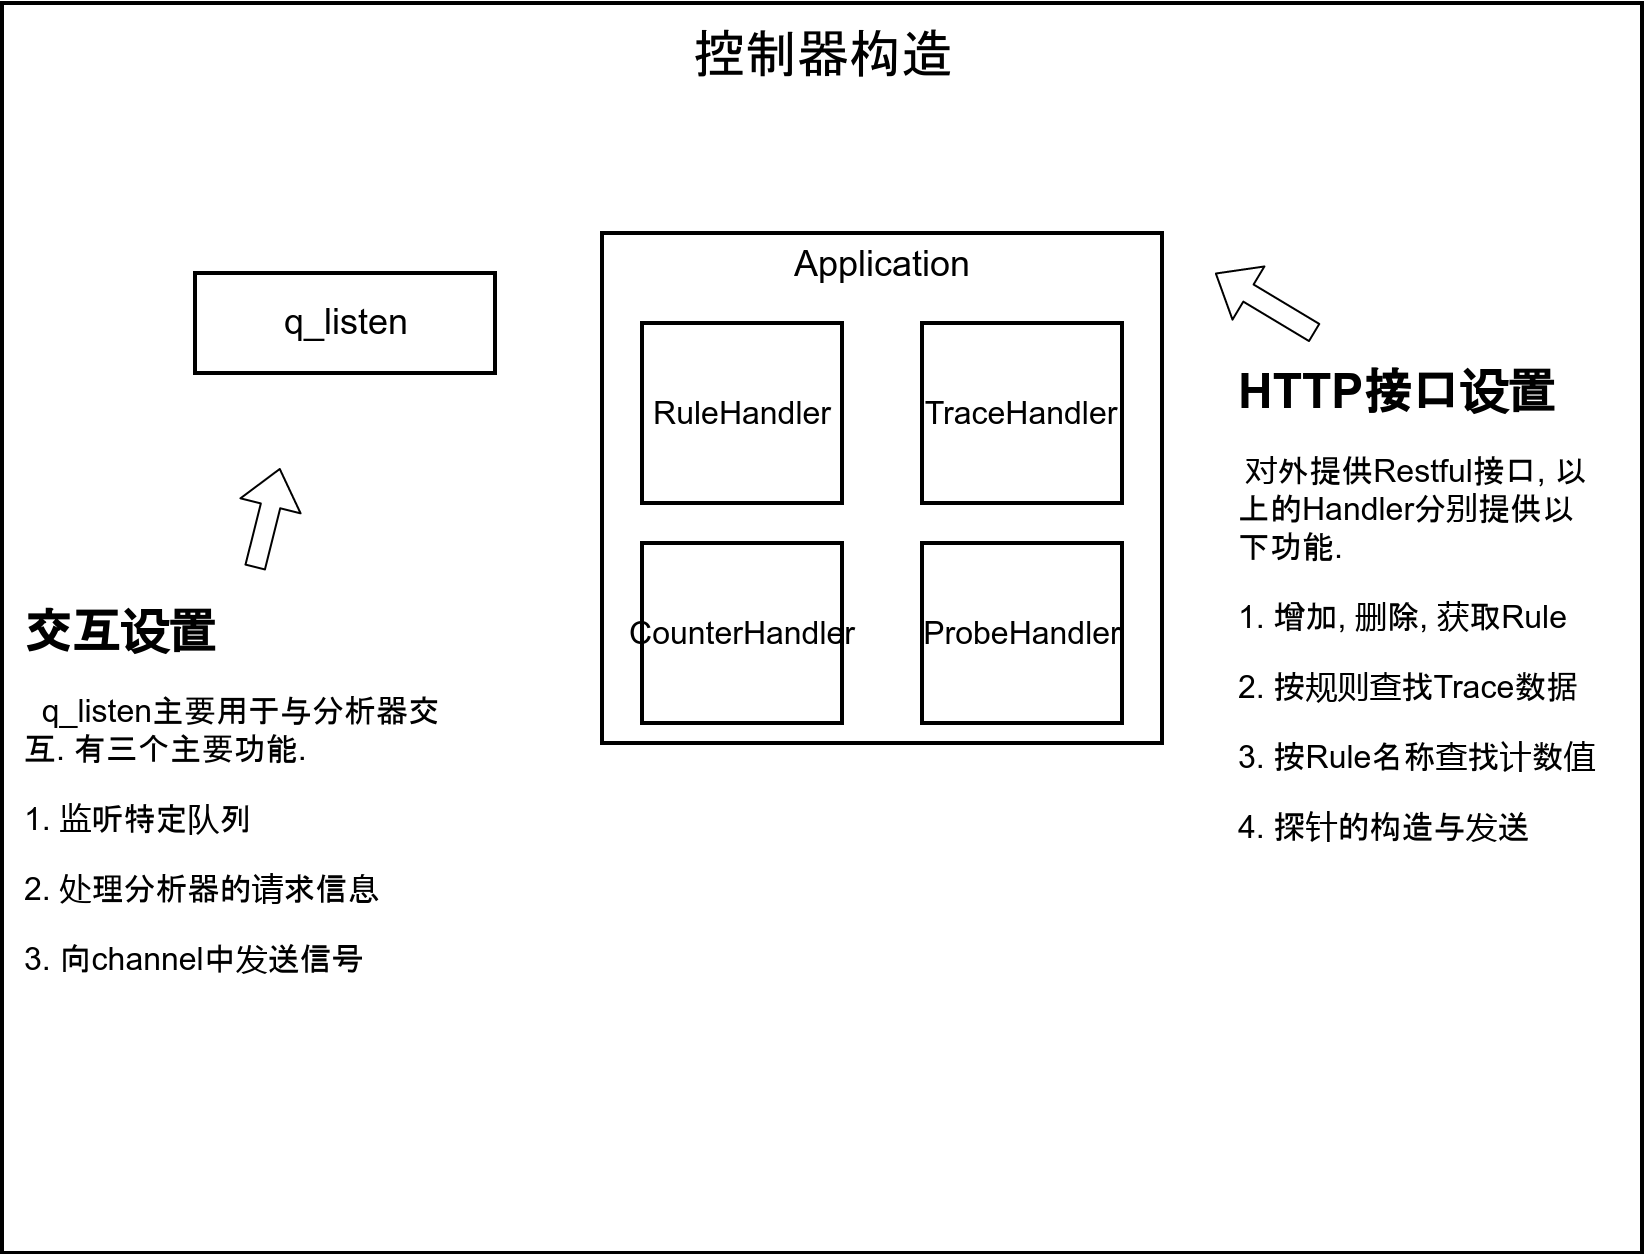
\includegraphics[width=0.9\textwidth]{../img/controler_arch.png}
  \caption{控制器构造}
  \label{fig:contoler_arch}
\end{figure}

控制器中, 涉及到三个方面:

\textbf{与存储器交互}: 我们的存储器使用\texttt{MySQL},
Python程序可以方便的进行读写; 允许用户读取Trace记录, 读取统计信息.
允许用户读写统计规则, 以及构造探针

\textbf{与分析器交互}: 通过\texttt{Redis}\cite{redis}进行解耦, 每个分析器启动时,
需要首先向控制器发送请求, 获得控制器的允许后, 才能启动.
如果用户更新了统计规则, 控制器也会立刻下发到所有的的分析器中.
在分析器准备结束时, 也同样需要告知控制器. 未来的控制器可能还需要添加
对于每个分析器的管理功能.

\textbf{与用户进行交互}: 通过访问页面发送请求, 进行交互. 采用基于HTTP协议的API,
程序功能也可以轻松的进行扩展.


\section{有关程序性能的问题}

  对于\texttt{CPython}来说, 由于全局中断锁也就是\texttt{GIL}的存在, \texttt{CPython}
无法充分的利用多核. 因此, 编写控制器时, 我选择单线程, 也因此选择了\texttt{Tornado}.

 不过所有用户均是在一个线程中进行轮转, 如果某个用户请求时间过久,
将会严重影响其他用户的查询体验.
% }}} 控制器的设计与实现

% {{{ 存储器与访问页面的设计与实现
\chapter{存储器与访问页面的设计与实现}

\section{存储器的设计与实现}

\subsection{数据库设计}
\label{sec:数据库设计}

\subsubsection{trace数据存储}

存储trace数据的库表分为三大部分:

\begin{itemize}
    \setlength\itemsep{0.1em}
    \item 第一部分是数据包原始信息, 包括数据包头部以及负载信息.
    \item 第二部分是每一跳的信息, 比如时间戳, 源MAC地址. 每个trace数据跳数不同,
            所以保存时, 将所有跳的信息结合在一起存储.
    \item 第三部分是元数据信息, 表示这个trace信息是否有环, 是否丢包,
            是否为探针数据.
\end{itemize}


\begin{table}[]
    \centering
    \caption{tbl\_traffic\_data}
    \begin{tabular}{llll}   \hline
    Field          & Type          & Comment                   \\ \hline
    id             & int(11)       &                           \\
    s\_ip          & int(11)       & 源IP                       \\
    d\_ip          & int(11)       & 目的IP                      \\
    protocal       & int(11)       & 协议类型                      \\
    generate\_time & timestamp     & 产生时间                      \\
    trace\_data    & varchar(1024) & trace数据信息, 保存为二进制字符串    \\
    fdate          & int(11)       & 存入日期, 如果数据量过大则使用索引 \\
    is\_loop       & int(11)       & 是否有环                      \\
    is\_drop       & int(11)       & 是否丢包                      \\
    is\_probe      & int(11)       & 是否为探针                    \\ \hline
    \end{tabular}
    \label{tbl_traffic_data}
\end{table}



\subsection{Counter计数器表格的设计}

存储计数器的数据表相对简单, 主要记录分析器ID, 计数值以及产生时间.

\begin{table}[]
    \centering
    \caption{tbl\_counter}
    \label{tbl_counter}
    \begin{tabular}{lll} \hline
    Field          & Type          & Comment \\ \hline
    id             & int(11)       &         \\
    counter\_name  & varchar(1024) & 计数器名称   \\
    generate\_time & timestamp     & 数据产生时间  \\
    analyer\_id    & int(11)       & 分析器ID   \\
    cnt            & int(11)       & 计数值     \\
    fdate          & int(11)       & 数据产生日期  \\ \hline
    \end{tabular}
\end{table}

目前的分析器中, 想要定时10s进行发送计数器信息, 所以一天的数据大约有
$$\frac{24 \times 3600 s}{10s} = 8640 Rows $$

如果我们有3台交换机的话, 10个计数规则的话, 每天将会有250,000条记录,
每个月大约有7,500,000条.

MySQL主要支持百万级别的数据, 因此, 在正式投入使用时,
整个程序需要使用分区表(按月分区).
如果有可能我们最好将粒度设置为20s, 可以减少一半的存储占用.

我建议数据保存时间最好不要超过1个月, 有了问题需要尽快解决.


\subsection{存储trace数据中路径信息的考量}

由于对于某个数据包的整条路径, 我们是需要进行存储的. 但是,
路径存储到数据库后, 我们不打算提供对于数据路径的检索功能. 这样,
可以将所有字段结合在一起放置在数据库中.

对于该字段, 曾经我考虑使用\texttt{Protobuf}与\texttt{JSON}两种.
最终选择了\texttt{JSON}, 主要有以下两个原因:

\begin{enumerate}
\def\labelenumi{\arabic{enumi}.}
\item
  \texttt{JSON}不只是在存储中用到了,
  在\texttt{Watcher}与控制器交互过程中, 也全部使用了\texttt{JSON}. 因此,
  使用\texttt{JSON}能减少项目依赖的类库数量.
\item
  \texttt{Protobuf}在存入数据库时, 需要采用特定的数据结构. 存入取出时,
  开发者并不容易使用肉眼调试分析.
\end{enumerate}

鉴于此, 我放弃了内存占用量较小的\texttt{Protobuf},
转而使用易于读取理解的\texttt{JSON}.


\section{访问页面设计与实现}

\subsection{访问页面设计}

下图\ref{fig:traffic_data_show}, \ref{fig:counter_data_show}
分别展示了数据流量的显示以及计数器统计结果的显示,

\begin{figure}[htbp!]
  \centering
  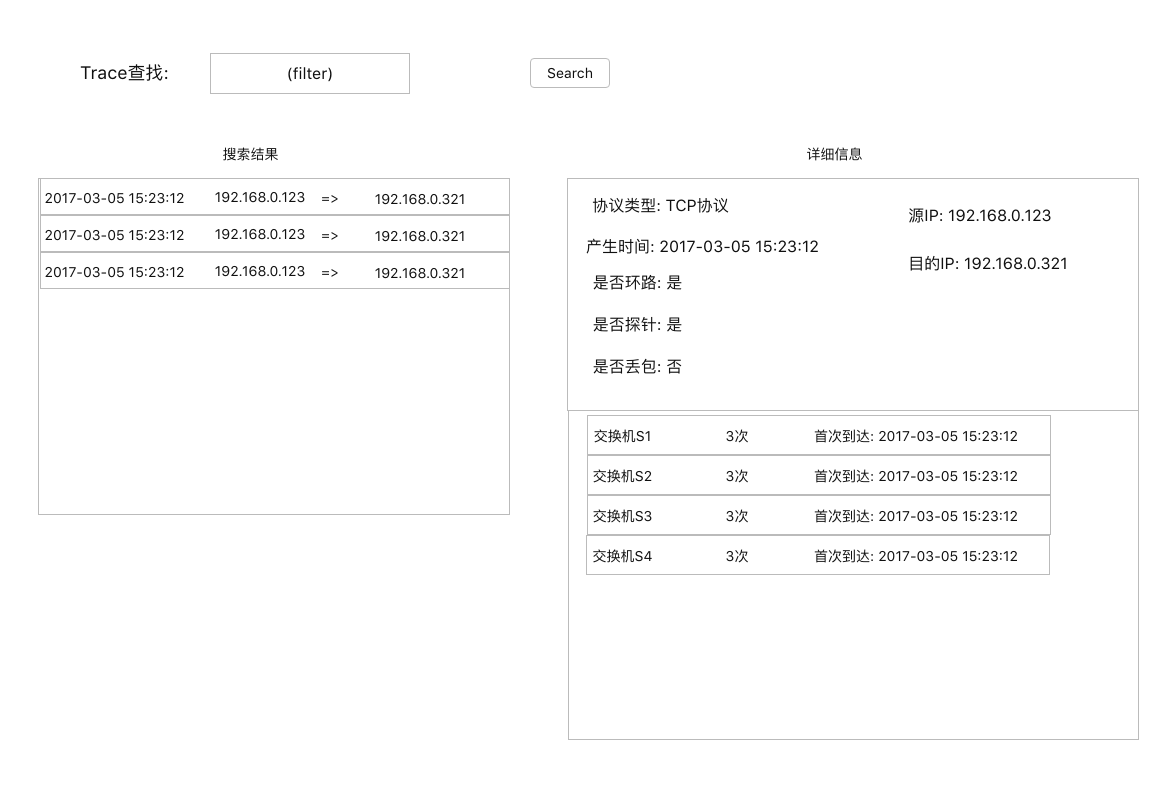
\includegraphics[width=0.9\textwidth]{../img/traffic_data_show.png}
  \caption{路径信息}
  \label{fig:traffic_data_show}
\end{figure}

\begin{figure}[htbp!]
  \centering
  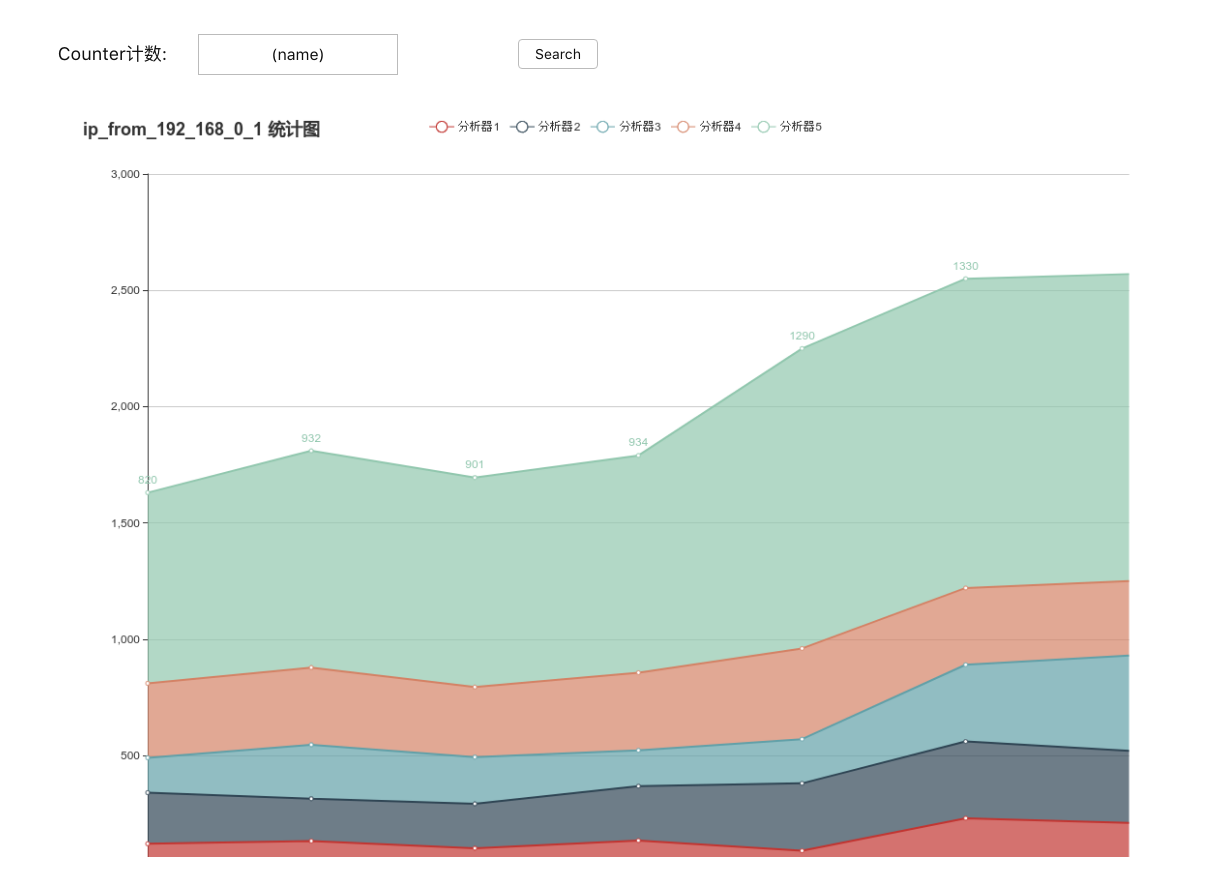
\includegraphics[width=0.9\textwidth]{../img/counter_data_show.png}
  \caption{计数器数据}
  \label{fig:counter_data_show}
\end{figure}

\subsection{有关预警方式选择}

  预警也是本程序应有的功能, 为了开发方便, 以及未来其他接入功能的使用,
我采用了\texttt{PushBear}服务, 用户可以直接扫描二维码关注预警频道.
而后将会收到预警信息. 用户可以在任意时刻取消订阅.

\begin{figure}[htbp]

\centering
\begin{minipage}{0.76\textwidth}

    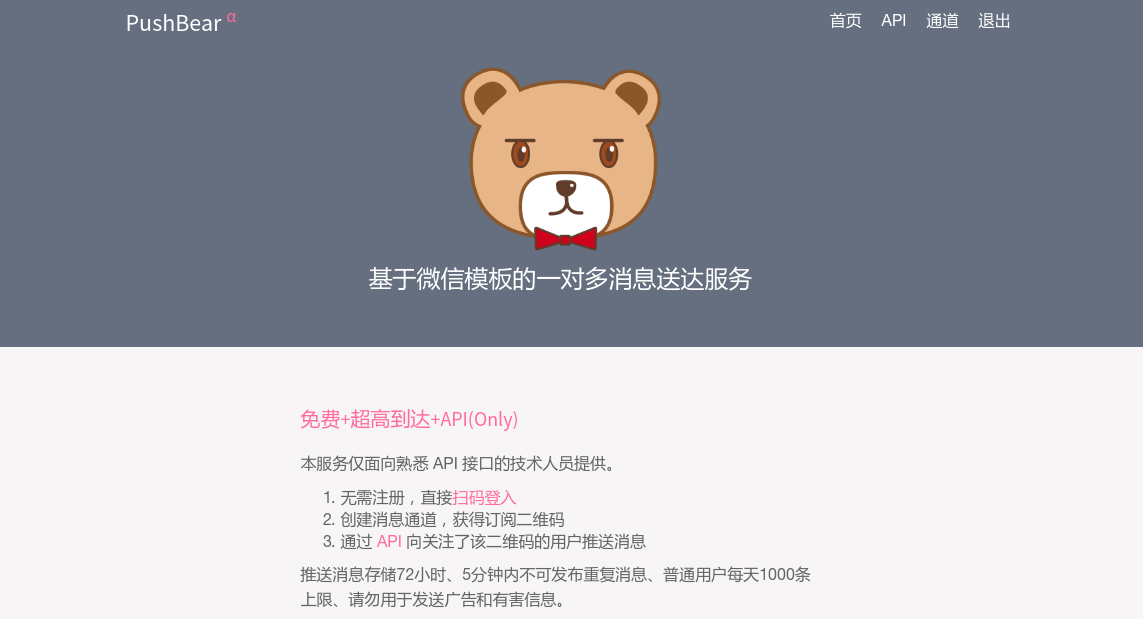
\includegraphics[width=1\textwidth]{../img/pushbear.png}
    \caption{PushBear官网}
    \label{fig:pushbear}

\end{minipage} \hfill
\begin{minipage}{0.22\textwidth}

\centering
    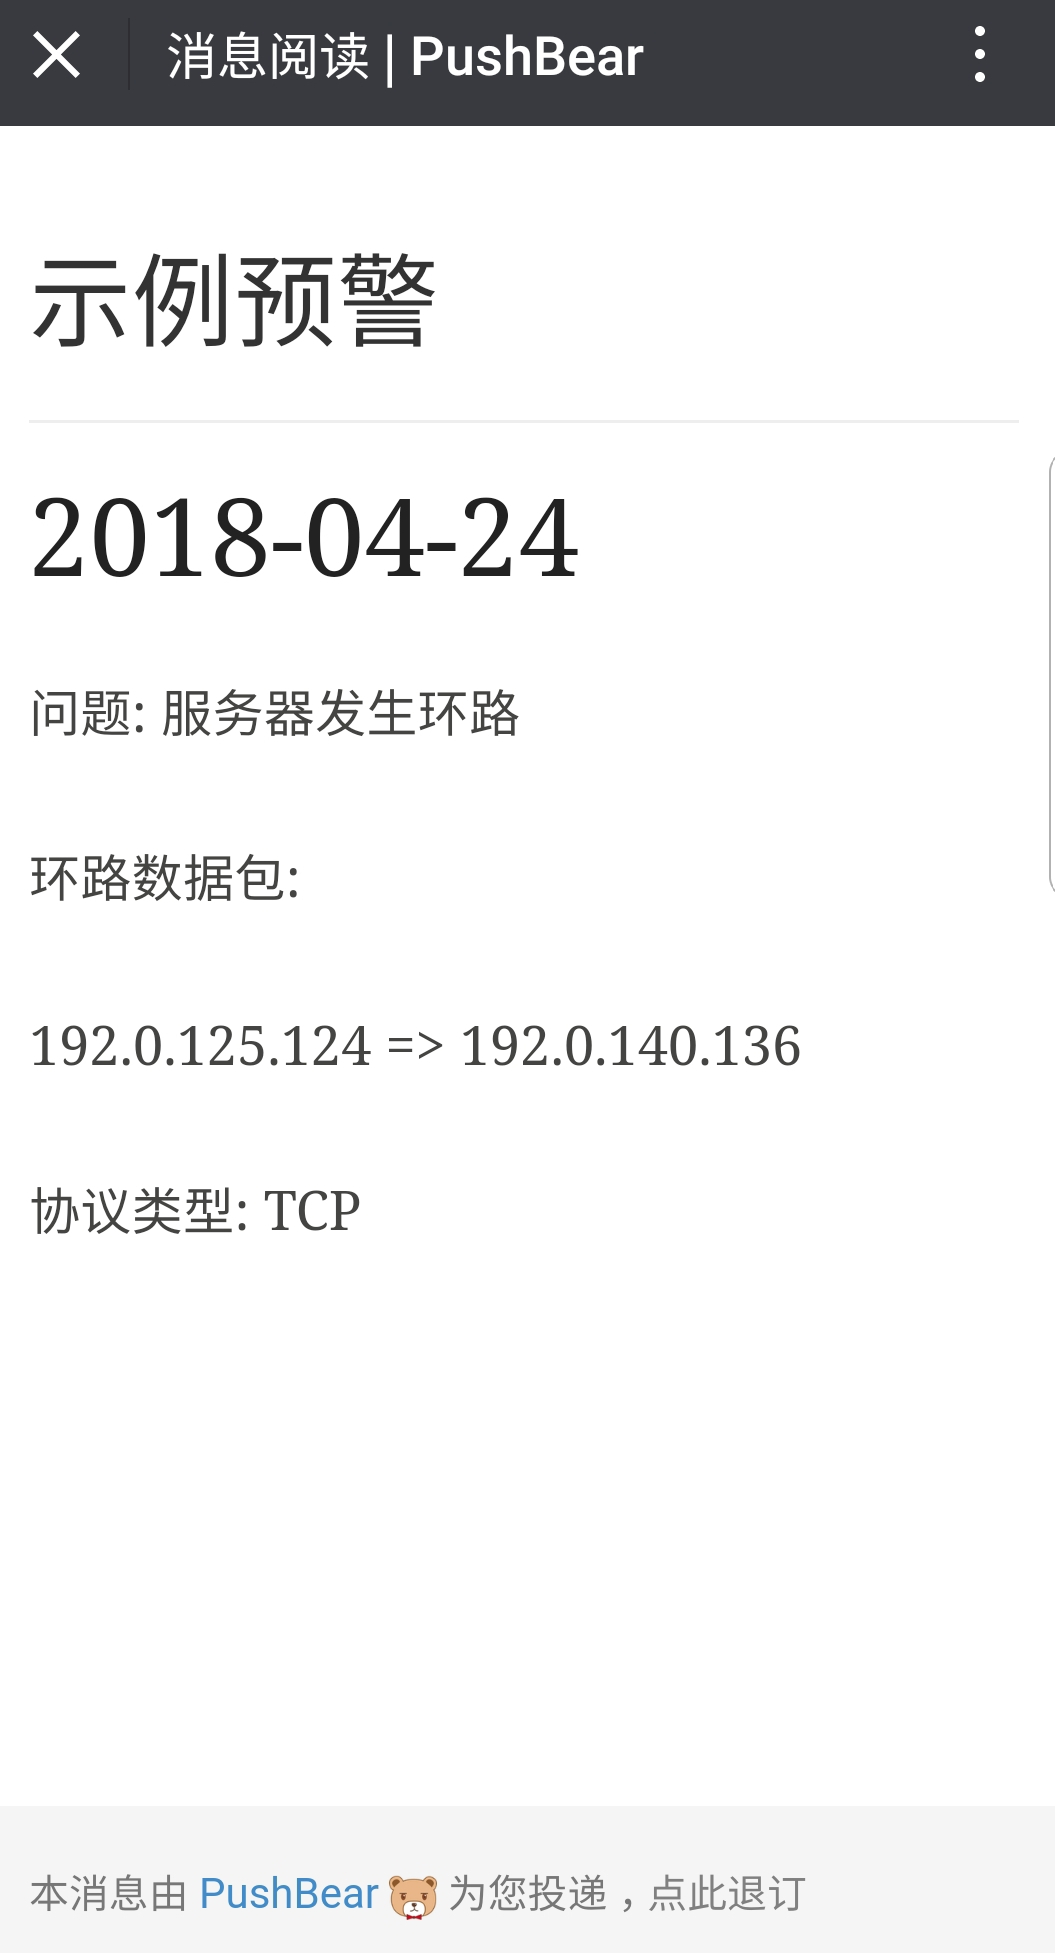
\includegraphics[width=1\textwidth]{../img/push_example.jpg}
    \caption{推送样例}
    \label{fig:push_example}
\end{minipage}

\end{figure}

如图\ref{fig:pushbear}为官网, 右侧\ref{fig:push_example}为推送样例.

%  https://pushbear.ftqq.com/admin/#/
% }}} 存储器与访问页面的设计与实现

% }}} 实现方案

%  {{{ 程序部署与性能评测
\chapter{程序部署与性能评测}
\section{程序部署}

  本次的程序设计主要分为三个部分, 分析器, 存储器以及控制器, 展示页面由控制器
负责加载. 承接上文分析器控制接口设计\ref{sec:分析器, 控制器接口设计}, 分析器, 
控制器, 与存储器之间是不存在耦合的, 均可进行单独的部署.

  它们之间唯一需要的只有TCP连接. 另外, 有关Redis服务器, 我选择将其与存储器放置在一台
服务器上. 最主要的原因就是Redis以及MySQL的存在, 就是为了连接分析器与控制器,
放置在一台服务器上符合它们的作用.

  分析器可以在多台PC进行部署, 这是由于一条路径上的所有数据包都会根据hash操作
分配至同一个分析器中. 可以利用这一特性, 进行横向扩展来提高系统的吞吐量.

  有关详细的部署操作, 在代码的文档\texttt{README}\cite{Niftyflow}中均有记录,
在此不进行赘述.

\section{评测要点与评测环境}

  程序中, 实现的功能有下面这些:

\begin{itemize}
    \item 对分析器: 包括有网卡数据读取, 快慢路径处理数据, 有问题的trace数据入库,
计数器报告, 报警信息发送.
    \item 对存储器: 读写有问题的trace数据, 读写计数值.
    \item 对控制器: 分析器的初始化, 提供数据访问接口, 添加删除规则, 探针的发送.
\end{itemize}

  对于存储器来说, 只负责存储异常的数据包信息以及提供访问能力, 建立合适的索引之后,
数据库可以保持较好的性能. 控制器只负责控制分析器与提供接口, 数据量并不大.
三者中对性能要求较高的部分为分析器, 尤其是数据包的读取与处理能力, 决定着整个
程序的吞吐量, 测试的主要工作也只针对分析器.


测试环境的服务器配置如表\ref{tbl:server_config}所示.

\begin{table}[]
    \centering
    \caption{服务器配置}
    \label{tbl:server_config}
    \begin{tabular}{ll} \hline
    Field    & Type          \\
    Linux发行版 & CentOS 7.4 \\
    内核版本   &   3.10.0 \\
    CPU:     & Intel(R) Xeon(R) CPU E5-2690 v4 @ 2.60GHz(28核) \\
    内存:    & 32G                                       \\
    数据来源 & 使用pcap监听lo 采用tcpreplay指定测试数据以及发送速率. \\ \hline
    \end{tabular}
\end{table}


\section{评测过程}

\begin{itemize}
    \item 首先启动分析器程序
    \item tcpreplay进行大量的数据包发送, 评测时的输入3,000,000pps(packets per second).
    \item 评测大概进行了5分钟, 而后我将程序关闭并退出.
\end{itemize}

\section{评测结果及分析}

 下面两张图对应的均为日志记录为\texttt{INFO}的情况. 对于日志记录为\texttt{DEBUG}
的情况, 生成的日志过于庞大, IO占了很大一部分性能, 要比INFO时的性能损失一些.

\begin{figure}[htbp!]
  \centering
  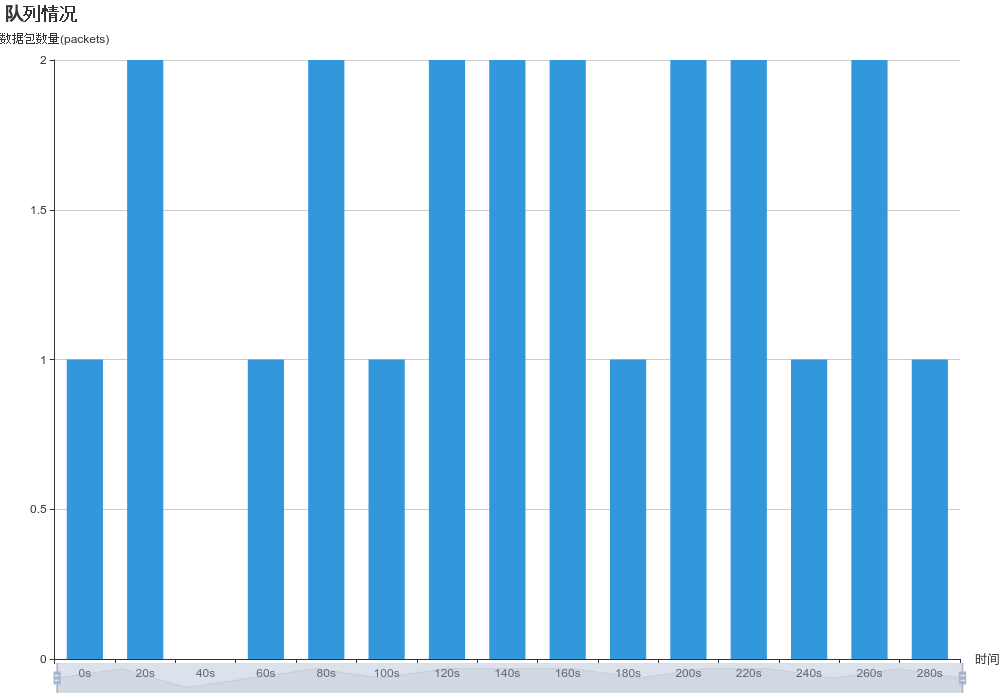
\includegraphics[width=0.8\textwidth]{../img/队列情况-new.png}
  \caption{队列中数据变化}
  \label{fig:queue_pic}
\end{figure}

\begin{figure}[htbp!]
  \centering
  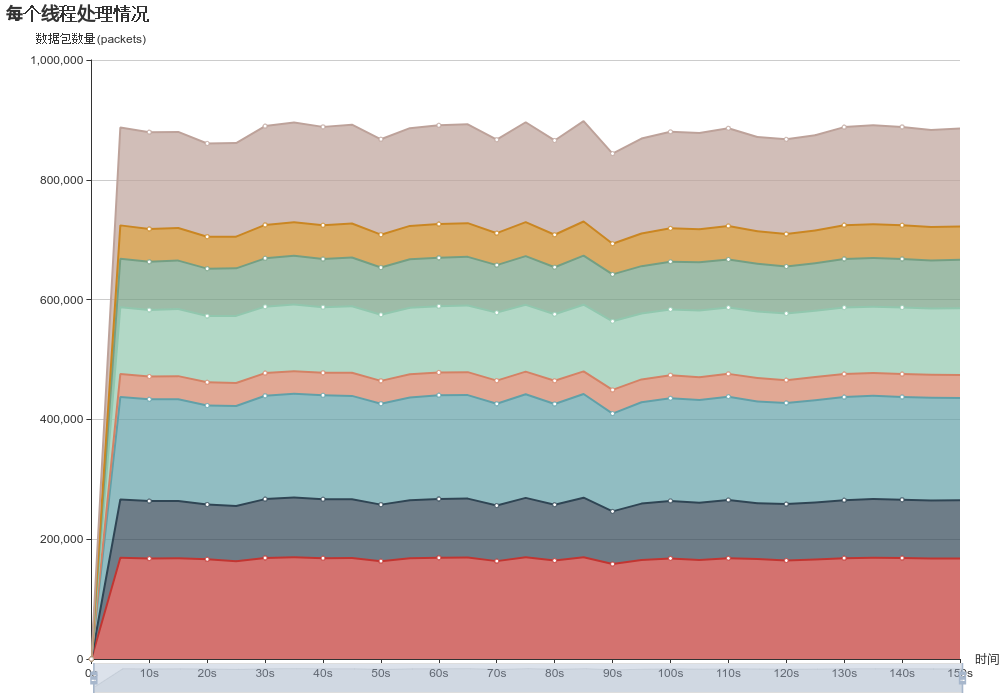
\includegraphics[width=0.8\textwidth]{../img/每个线程处理情况-new.png}
  \caption{各个线程处理情况}
  \label{fig:process_pic}
\end{figure}


通过观察\ref{fig:queue_pic}, 可以看得出, 使用lo进行数据接收时, 队列中的数据量
根本不会上升. 这也就说明了一点, 当前程序的瓶颈是在\texttt{pcap\_open\_live}阶段.
这里我只测试了\texttt{pcap}库, 未来如果改用\texttt{dpdk}或许能达到更好的效果.

通过观察\ref{fig:process_pic}, 所有process线程的处理速度基本是稳定的,
处理速度上的不同, 原因只是hash函数选择的问题. 某些线程被分到了比较多的数据包.
也可以看的出, 当前的处理速率大概是88万pps, 也就是平均每个线程有10万pps.
这里并不是说单个线程的处理只有10万pps, 只能说明, 我们每秒到达的数据包只有这么多.

具体的评测过程以及日志分析脚本请查看
\texttt{analyzer/README.md}\cite{Niftyflow}中的性能评测部分,我介绍了相对详细的评测过程以及结果分析.

% }}} 程序部署与性能评测

\chapter{总结与展望}

\section{论文总结}

  本次的设计, 实现了一个针对大型DCN的可扩展数据包级检测系统, 基于商用交换机的
"匹配镜像"机制, 可以获取捕获DCN中的数据包, 以及发送探针重现数据包的路径.
项目也有详细的部署文档, 可以快速部署到DCN中, 同时, 也提供了查询和配置接口.

  在微软提出Everflow设计时, 并没有开放源代码, 当前的市面上也没有针对Everflow的
开源实现. 本次的设计也填补了这项空白, 整个项目作为开源工程, 接受大家的检验并
提供支持.

  实验室中基于专有硬件平台的分析工具正在实现中. 此次我的毕业设计, 实现了最初提出的
功能后, 对程序性能也进行了简单评估, 为实验室的工作提供了一份参照.

\section{工作展望}

  目前的工作中, 是在数据包读入部分存在瓶颈, 未来, 可能会使用\texttt{dpdk}
以及\texttt{RSS}(Receive side scaling)\cite{rss}机制, 允许一个分析器使用多个CPU
核接受数据包.

  目前的部署只在单台DCN中进行了部署, 程序的鲁棒性以及数据处理能力还有待进一步
测试. 程序中的内存泄露问题已经解决(使用Valgrind\cite{Valgrind}),
但从我的调研结果来看, 针对\texttt{DPDK}程序进行内存泄露检测时,
\texttt{Valgrind}需要打补丁进行编译, 所以\texttt{DPDK}程序的内存安全性不能保证.
这些工作待有了真实环境之后, 可以着手开始. 当前对于错误信息, 程序需要通知运维人员进行处理,
未来, 也会为程序增加自动化的错误探测功能, 主动解决网络问题并生成报告.
